\documentclass{amsart}

\usepackage{fullpage, amsmath, amssymb, amsthm, tabularx, multirow, multicol, tikz, venndiagram, graphicx}
\renewcommand{\baselinestretch}{1.15}

\title{Math Concepts_2_Functions}
\author{Emre Usenmez}
\thanks{Gonville \verb|&| Caius College. Extremely grateful to Prof Jay Cummings as these notes made liberal use of his book 'Proofs'.}
\date{August 2023}

\newtheorem{thm}{Theorem}
\theoremstyle{definition}
\newtheorem*{dfn}{Definition}
\theoremstyle{definition}
\newtheorem*{prpn}{Proposition}
\theoremstyle{remark}
\newtheorem*{note}{Note}

\usepackage{Sweave}
\begin{document}
\Sconcordance{concordance:Math_Concepts_2_Functions.tex:Math_Concepts_2_Functions.Rnw:1 %
18 1 1 0 71 1}


\begin{center}
      \textbf{TOPIC TWO: FUNCTIONS}
\end{center}

In Topic One we studied the static properties of sets. Things get more dynamic when we start applying functions to those sets.

\section{\textbf{Definitions}}
\begin{dfn}
      \boxed{f:A \rightarrow B} \quad Given a pair of sets $A$ and $B$, suppose that each element $x \in A$ is associated, in some way, to a unique element of $B$, which we denote $f(x)$. Then $f$ is said to be a \emph{function} from $A$ to $B$. This is often denoted
      \[ f: A \rightarrow B \]
      which is typically read "$f$ from $A$ to $B$."
      \begin{flalign*} % used flalign instead of align to left-justify the text and not center it. Lines within each flalign should begin and end with &.
            \text{Furthermore, }
            &A \text{ is called the \emph{domain} of } f, && \text{(can be though of as inputs of $f$)} & \\
            &B \text{ is called the \emph{codomain} of } f, \text{ and} && \text{(\dots as a set to which all outputs belong)} & \\
            &\text{The set } \{f(x):x \in A\} \text{ is called the \emph{range} of } f. && \text{(\dots as outputs of $f$)}
      \end{flalign*}
      All three correspond to each other via $f$ but they are just sets. \\
      Range consists only of elements in the codomain that gets mapped. That is, $y$ is in the range if there is an $x$ in the domain that maps to it: $f(x) = y$. For e.g.,
      \begin{itemize}
            \item if $f : \mathbb{R} \rightarrow \mathbb{R}$ is given by $f(x) = 2x$ then the range is $\mathbb{R}$.
            \item if $f : \mathbb{R} \rightarrow \mathbb{R}$ is given by $f(x) = x^2$ then the range is the set of nonnegative real numbers: ie, the interval $[0, \infty)$.
      \end{itemize}
\end{dfn}

A function's domain and codomain can each be any set. Here is a graphical way to write som function $f$:

\begin{figure}[h] %The optional argument to the figure environment tells LaTeX where you'd like it to appear, if possible; the options are h meaning "here", t (at the top of a page), b (at the bottom of a page) and p (on a page without any text). This is only a suggestion to LaTeX, and it might ignore it if it doesn't think your instruction can be done neatly. If you want to encourage LaTeX to take your suggestion seriously you can put an exclamation mark before the location, e.g. \begin{figure}[!b].
      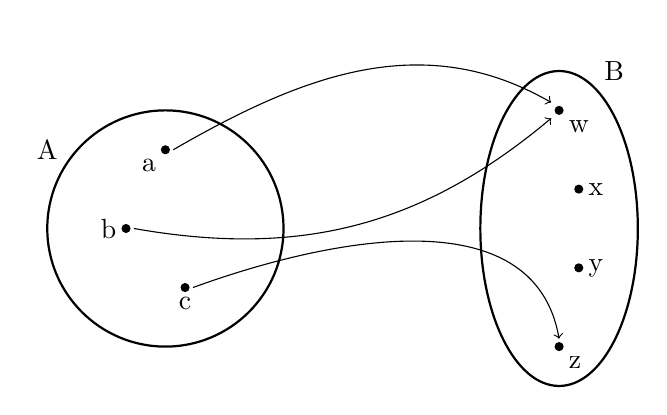
\begin{tikzpicture}
            \draw [thick] (1,0) circle (1.5cm); %This large circle contains points a, b, c
                  \node at (-0.5,1) {A}; % This produces the set name A
            \draw[thick] (6,0) ellipse (1cm and 2cm);
                  \node at (6.7,2) {B};

            \draw[fill] (1,1) circle [radius = 0.05]; %This is the dot we will label a
                  \node [below left] at (1,1) {a}; % We name the dot a and locate it below left of (1,1)
            \draw [fill] (0.5, 0) circle [radius = 0.05];
                  \node [left] at (0.5, 0) {b};
            \draw[fill] (1.25,-0.75) circle [radius = 0.05];
                  \node[below] at (1.25,-0.75) {c};

            \draw[fill] (6, 1.5) circle [radius = 0.05];
                  \node[below right] at (6, 1.5){w};
            \draw[fill](6.25, 0.5) circle [radius = 0.05];
                  \node[right] at (6.25, 0.5){x};
            \draw[fill](6.25, -0.5) circle [radius = 0.05];
                  \node[right] at (6.25, -0.5){y};
            \draw[fill](6, -1.5) circle [radius = 0.05];
                  \node[below right] at (6, -1.5){z};

            \draw[->] (1.1,1) to [out=30, in=150] (5.9, 1.6); % arrow from a to w with curve degrees.
            \draw[->] (0.6, 0) to [out=-10, in=220] (5.9, 1.4); % arrow from b to w with curve degrees.
            \draw[->] (1.35, -0.75) to [in=100, out=20] (6, -1.4); %arrow from c to z with curve degrees.
      \end{tikzpicture}
    \caption{A function $f: A \rightarrow B$}
            \label{fig:function_diagram} %allows us the refer to this figure later on even if the figure numbering changes it keeps references correct.
\end{figure}

Figure \ref{fig:function_diagram} above illustrates a function with \emph{domain} \{a, b, c\}, \emph{codomain} \{w, x, y, z\}, and \emph{range} \{w, z\}.
\begin{note}
      There does not exist any $k \in \{a, b, c\}$ such that $f(k)=y$, which is why $y$ is not in the range.
\end{note}

For diagrams such as Figure \ref{fig:function_diagram} to represent a function, it would have to satisfy both existence and uniqueness aspects of a function. If it fails to do so, then it would not represent a function. For e.g., if $b$ did not map onto any of the elements in $B$ in Figure \ref{fig:function_diagram} then the diagram would not satisfy the existence condition - since $b$ is being sent to nowhere - and thus not represent a function. Similarly, if $b$ not only mapped onto $w$ but also onto $y$ simultaneously then it would not satisfy the uniqueness condition and the diagram would again not represent a function.




\end{document}
